\documentclass{beamer}
\usepackage[spanish]{babel}
\usepackage[utf8]{inputenc}
\usepackage{booktabs}
\usepackage{graphicx}

\usetheme{Berkeley}

\newcommand{\spaced}{\hspace{.2cm}}


\title{Filtrado de ruido en imagenes con transformada de Wavelet}
\author{
  G.Isaias $^1$ \and   
  M.Santiago $^2$ \and 
  S.Lautaro Andres $^3$ \and
  V.Xavier $^4$ 
}
\institute{
  $^{1-2-3-4}$ Universidad Nacional del Comahue \\ 
  Buenos Aires , Neuquen \\ 
}
\date{}

\begin{document}
    
  \begin{frame}
    \titlepage  
  \end{frame}

  \begin{frame}
    \tableofcontents
  
    
  
  \end{frame}

  \section{Resumen}

  \begin{frame}
    \frametitle{Resumen}
    
    Resumen del trabajo ( alguna imagen que represente nuestro trabajo )
    Sugerencia usar a lenna
  
  \end{frame}

  \section{Marco Teorico}
  \subsection{Analisis Multiresolucion}
  
  
  \begin{frame}
   \frametitle{ Análisis Multiresolución }
   Un análisis multiresolución para $L^{2}(\mathbb{R})$ consiste en una secuencia de subespacios cerrados de $L^{2}(\mathbb{R})$, $\{ V_{j} \}_{j \in \mathbb{Z} }$, una función  una función $\phi \in V_{0}$ tal que se cumplan las siguientes condiciones:

   \begin{itemize}
   \item[i.] Los espacios $V_{j}$ están anidados, es decir:
   \begin{equation*}
   ... \subset V_{-1} \subset V_{0} \subset V_{1} ...
   \end{equation*}
   \item[ii.] $\overline{\cup _{j\in \mathbb Z}V_j} = L^2(\mathbb R)$ y $\cap {j\in \mathbb Z}V_j = {0}$
   \item[iii.] Para todo $j \in \mathbb{Z}$, $V_{j-1}=D(V_j)$
   \item[iv.] $f \in V_0 \rightarrow T_kf \in V_o$, $\forall k \in \mathbb{Z}$
   \item[v.] $\{T_k \phi \}_{k \in \mathbb{Z}}$ es una base ortonormal de $V_0$
   \end{itemize} 
  \end{frame}
\begin{frame}
  \frametitle{Análisis Multiresolución}
 Se define a $W_j$ como el complemento ortogonal de $V_j$ en $V_{j-1}$
  \begin{equation}
    \label{Central}
    V_{j-1} = V_j \oplus W_j
  \end{equation}
  \begin{equation}
    \label{NivApDet}
    A_{j-1}(t) = A_j(t) + D_j(t) 
  \end{equation} 
Por otro lado:
\begin{equation}
  V_J = V_K \oplus W_K \oplus ... \oplus W_{J+1}, \: J<K
  \label{eq.Vj}
  \end{equation}
Finalmente:
\begin{equation}
  x(t) = A_J(t) + \sum_{j=-\infty}^{J}D_j(t)
  \end{equation}

\end{frame}
\begin{frame}
\frametitle{Análisis Multiresolución}
$\rightarrow$ Vemos ejemplo en el toolbox de Matlab
  
Para continuar:
\begin{itemize}
  \item 
  \begin{equation}
    A_j(t)=\sum_{k \in \mathbb Z} \beta _{j,k} \phi _{j,k}(t)
  \end{equation}
  Donde:
  \begin{equation}
    \label{Beta}
    \beta _{j,k}= <x(t), \phi _{j,k}(t)>
  \end{equation}

  \item
  \begin{equation}
    D_j(t)=\sum_{k \in \mathbb Z} \alpha _{j,k} \psi _{j,k}(t)
  \end{equation}
  Donde:
  \begin{equation}
    \label{Alfa}
    \alpha _{j,k}= <x(t), \psi _{j,k}(t)>
  \end{equation}
\end{itemize}
La función $\psi \in L^{2}(\mathbb{R})$ y $\{T_k \psi \}_{k \in \mathbb{Z}}$ son una base ortonormal de $W_0$
\end{frame}

\begin{frame}
\subsection{Umbralización}
\frametitle{Umbralización}
\centering
\begin{figure}[htb]
  \centering
  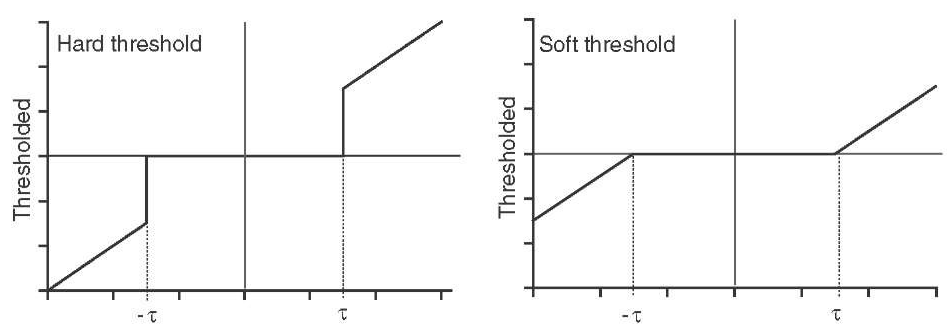
\includegraphics[scale=0.4]{imgs/Umbral}
  \caption{Modos de umbralización más utilizados}
  \label{}
\end{figure}
\end{frame}

\begin{frame}
  \frametitle{Umbralización}
Algortimos para el cálculo del umbral $\tau$:
\begin{itemize}
  \item VisuShrink
  \item LevelShrink
  \item BayesShrink
  \item NormalShrink
  \item AWT(Adaptative Wavelet Treshholding)
\end{itemize}
  

\end{frame}




  \section{Implementacion}

  \begin{frame}
    \frametitle{Pseudocodigo parametros optimos}
  
    \begin{itemize}
      \item Leer todas las imagenes de una carpeta.
      \item Agregar ruido gaussiano con $\mu=0$ y varianza $\sigma$.
      \item Seleccionar el parametro a variar, y dejar constante el resto de parametros.
      \item Transfromar la imagen utilizando la trasnformada de Wavelet.
      \item Calcular los umbrales para cada nivel segun el umbral seleccionado.
      \item Aplicar el modo (soft - hard) y eliminar las componentes menores al umbral.
      \item Aplicar la antitransformada.
      \item Calcular el PSNR y el SSIM.
    \end{itemize}
  
  \end{frame}

  \begin{frame}
    \frametitle{Pseudocodigo comparacion de filtros}
    \begin{itemize}
      \item 
    \end{itemize}
    
  
  \end{frame}

  \subsection{Banco de filtros}
  
  \begin{frame}
    \frametitle{¿Comó solucionamos el inconveniente del producto interno?}
    
    Estrategia: Algoritmo que relacione las bases ortonormales y la idea de banco de filtros.
      
     Si partimos de la ecuación \ref{Central} y recordamos como se descomponían estas funciones, tenemos el inconveniente de los productos internos.
        
  \end{frame}

   \begin{frame}

Reescribiendo la ecuación \ref{Central} 
   \begin{equation}
\label{Aj}
A_j(t)=\sum_{k \in \mathbb Z}  a^{j}_{k} \phi _{j,k}(t)
\end{equation} 
\begin{equation}
\label{Dj}
D_j(t)=\sum_{k \in \mathbb Z}  d^{j}_{k} \psi _{j,k}(t)
\end{equation} 
con
\begin{equation}
\label{ajk}
a^{j}_{k}= <A_{j}(t), \phi _{j,k}(t)>
\end{equation}
\begin{equation}
\label{ajk}
d^{j}_{k}= <A_{j}(t), \psi _{j,k}(t)>
\end{equation}
    \end{frame}
    
  \begin{frame}
   Podemos obtener $a^{j}$y $d^{j}$ a partir de $A_{j-1}$, partiendo de del 	producto interno de $A_{j-1}$ y las funciones de escala y wavelet
   \begin{equation}
<A_{j-1}(t),\psi _{j,k}(t)>=<A_{j}(t)+D_{j},\psi _{j,k}(t)>
\end{equation}

\begin{equation}
<A_{j-1}(t),\phi _{j,k}(t)>=<A_{j}(t)+D_{j},\phi _{j,k}(t)>
\end{equation}
  \end{frame}
  
  \begin{frame}
  A su ves sabemos que 
  \begin{equation}
  A_{j-1}(t)=\sum_{k \in \mathbb{Z}} a^{j-1}_{k} \phi^{j-1}_{k}(t)
  \end{equation}
  con lo que obtenemos que 
  \begin{equation}
  a^{j}_{k}=\sum_{p \in \mathbb{Z}} a^{j-1}_{p} <\phi_{j-1,p},\phi_{j,k}>
  \end{equation}
  \begin{equation}
  d^{j}_{k}=\sum_{p \in \mathbb{Z}} a^{j-1}_{p} <\phi_{j-1,p},\psi_{j,k}>
  \end{equation}
  \end{frame}
  
  \begin{frame}
  Pero tanto los productos internos de $<\phi_{j-1,p},\phi_{j,k}>$ $<\phi_{j-1,p},\psi_{j,k}>$, son productos internos de funciones conocidas que ya fueron calculadas por lo cual podríamos tomarlo como coeficientes conocidos mas aun como coeficientes de filtros.
  
\begin{equation}
	\sqrt{2} a_{p-2k}=<\phi _{j-1,p}(t),\phi _{j,k}(t)>
\end{equation}
	
\begin{equation}
	\sqrt{2} b_{p-2k}=<\phi _{j-1,p}(t),\psi _{j,k}(t)>
\end{equation}
  
  \end{frame}
\begin{frame}
Por lo que se definen los coeficientes de los filtros 
\begin{equation}
[LD]_{n}=\sqrt{2}  a_{-n}
\end{equation}

\begin{equation}
[HD]_{n}=\sqrt{2}  b_{-n}
\end{equation}
Donde LD es un filtro pasa bajos y HD es un filtro pasa altos.
Por lo que reescribimos a $a^{j}_k$ y $d^{j}_k$
\begin{equation}
\label{afinal}
a^{j}_{k}=\sum_{p \in \mathbb Z} a^{j-1}_{p} [LD]_{2k-p}
\end{equation}

\begin{equation}
\label{dfinal}
d^{j}_{k}=\sum_{p \in \mathbb Z} a^{j-1}_{p} [HD]_{2k-p}
\end{equation}

\end{frame}
\begin{frame}
Graficamente lo visualizamos
\begin{figure}[htb]
	\centering
	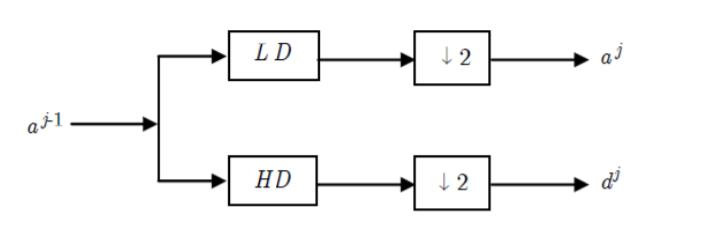
\includegraphics[width=.75\textwidth]{imgs/bancofiltros1D}
	\caption{Descomposición con banco de filtros para 1D.}
	\label{bancofiltros1D}
\end{figure}
\end{frame}
\begin{frame}
Para el caso que nosotros estudiamos, de imágenes, la descomposición en 2D, ve como un doble filtrado
\begin{figure}[H]
	\centering
	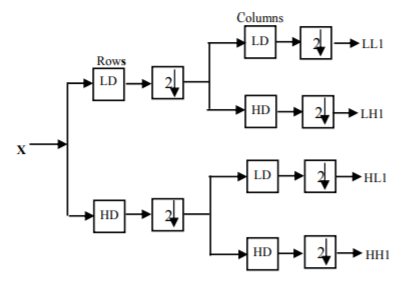
\includegraphics[width=.75\textwidth]{imgs/bancofiltros}
	\caption{Descomposición con banco de filtros para 2D.}
	\label{bancofiltros}
\end{figure}
\end{frame}
\begin{frame}
Es posible realizar el proceso inverso y recuperar la señal original
\begin{figure}[H]
	\centering
	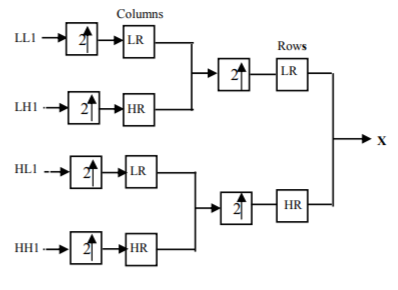
\includegraphics[width=.75\textwidth]{imgs/bancofiltrosR}
	\caption{Recomposición con banco de filtros para 2D.}
	\label{bancofiltrosR}
\end{figure}
\end{frame}






  \section{Resultados}

  \subsection{Imagenes de prueba}

  \begin{frame}
  
    Imagenes con ruido gaussiano con $\sigma=0.3$
  \end{frame}

  \subsection{Parametros optimos}

  \begin{frame}
    \frametitle{ Comparacion de Niveles }
    \centering
    \begin{tabular}{lrrrrr}
      \toprule
      {PSNR} &  noise &      1 &      2 &      4 &      6 \\
      \midrule
      Lenna &  17.65 &  23.92 &  \bf{27.03} &  22.29 &  22.29 \\
      House &  19.87 &  22.90 &  \bf{25.58} &  24.57 &  23.51 \\
      Wave &  18.63 &  23.34 &  \bf{26.70} &  24.71 &  24.65 \\
      \bottomrule
      \end{tabular}
  
      \begin{tabular}{lrrrrr}
        {SSIM} &  noise &      1 &      2 &      4 &      6 \\
        \midrule
        Lenna &  0.518 &  0.742 &  \bf{0.856} &  0.847 &  0.808 \\
        House &  0.620 &  0.806 &  \bf{0.882} &  0.839 &  0.814 \\
        Wave &  0.586 &  0.761 &  \bf{0.839} &  0.820 &  0.803 \\
        \bottomrule
        \end{tabular}

  \end{frame}

  \begin{frame}
    \frametitle{ Comparacion de Niveles }
    \centering
    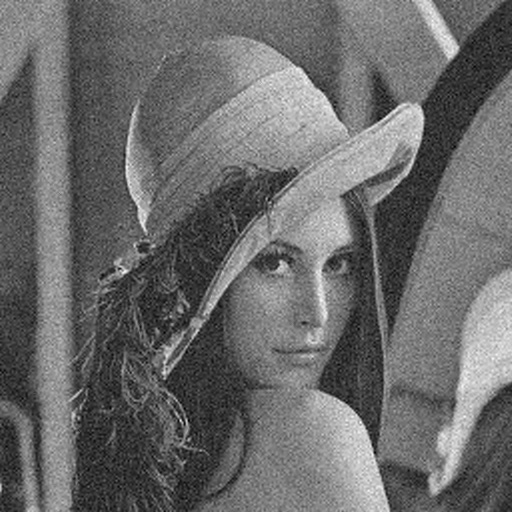
\includegraphics[width=3.5cm]{imgs/Levels/1_normal_soft_sym8_Lenna.jpg}
    \spaced
    \includegraphics[width=3.5cm]{imgs/Levels/2_normal_soft_sym8_Lenna.jpg}
    \\
    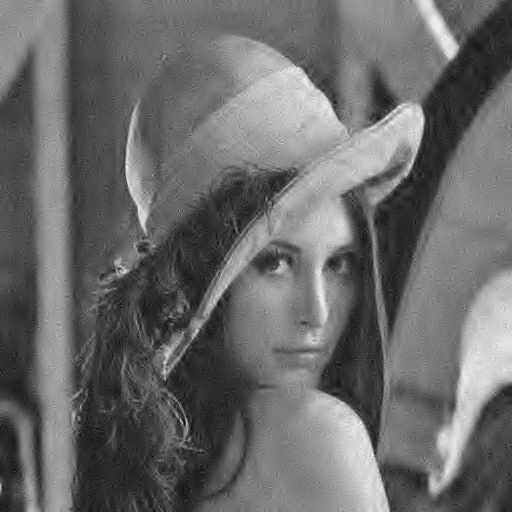
\includegraphics[width=3.5cm]{imgs/Levels/4_normal_soft_sym8_Lenna.jpg}
    \spaced
    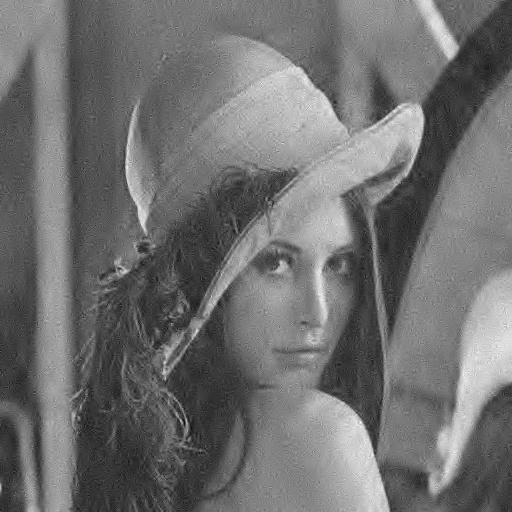
\includegraphics[width=3.5cm]{imgs/Levels/6_normal_soft_sym8_Lenna.jpg}
  
  \end{frame}

  \begin{frame}
    \frametitle{ Comparacion de modos }
    \centering
    \begin{tabular}{lrrr}
      \toprule
      {PSNR} &  noise &   soft &   hard \\
      \midrule
      Lenna &  17.65 &  \bf{27.03} &  21.41 \\
      House &  19.87 &  \bf{25.58} &  20.20 \\
      Wave &  18.63 &  \bf{26.70} &  20.85 \\
      \bottomrule
      \end{tabular}
      \begin{tabular}{lrrr}
        {SSIM} &  noise &   soft &   hard \\
        \midrule
        Lenna &  0.518 &  \bf{0.856} &  0.757 \\
        House &  0.620 &  \bf{0.882} &  0.789 \\
        Wave &  0.586 &  \bf{0.839} &  0.755 \\
        \bottomrule
        \end{tabular}

  \end{frame}

  \begin{frame}
    \frametitle{ Comparacion de modos }
    \centering
    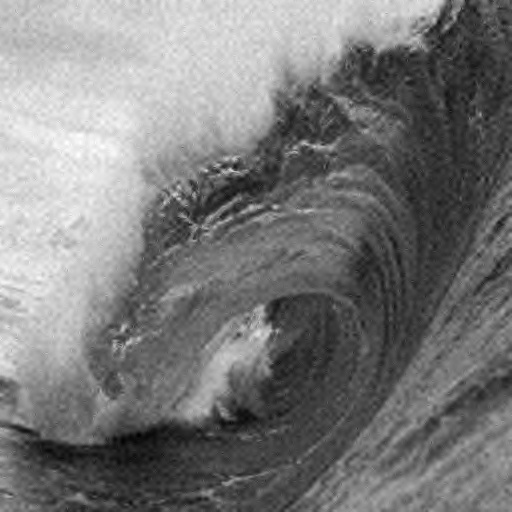
\includegraphics[width=5cm]{imgs/Modes/2_normal_soft_sym8_Wave.jpg}
    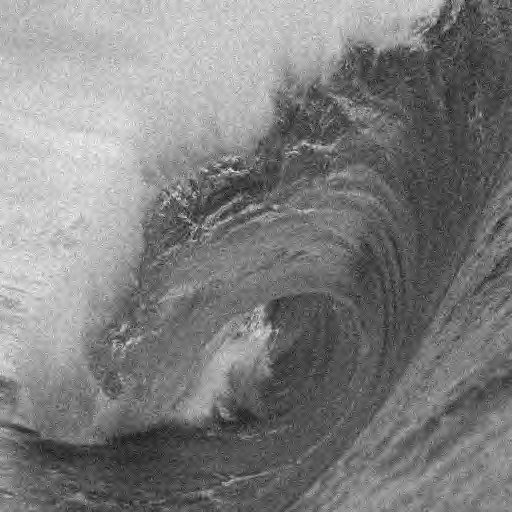
\includegraphics[width=5cm]{imgs/Modes/2_normal_hard_sym8_Wave.jpg}

  \end{frame}

  \begin{frame}
    \frametitle{ Comparacion de umbrales }
    \centering
    \begin{tabular}{lrrrrrr}
      \toprule
      {PSNR} &  noise &  universal &  bayes &  level &  normal &    awt \\
      \midrule
      Lenna &  17.65 &      25.86 &  25.71 &  25.40 &   \bf{27.03} &  25.24 \\
      House &  19.87 &      22.91 &  23.32 &  23.19 &   \bf{25.58} &  23.41 \\
      Wave &  18.63 &      26.74 &  26.70 &  26.86 &   \bf{26.70} &  25.56 \\
      \bottomrule
      \end{tabular}
      \begin{tabular}{lrrrrrr}
        {SSIM} &  noise &  universal &  bayes &  level &  normal &    awt \\
        \midrule
        Lenna &  0.518 &   0.848 &  0.847 &  0.849 &  \bf{0.856} &  0.838 \\
        House &  0.620 &   0.851 &  0.850 &  0.857 &  \bf{0.882} &  0.849 \\
        Wave &  0.586 &   0.830 &  0.829 &  0.833 &  \bf{0.839} &  0.823 \\
        \bottomrule
        \end{tabular}



  \end{frame}

  \begin{frame}
    \frametitle{ Comparacion de umbrales }
  
    \centering
    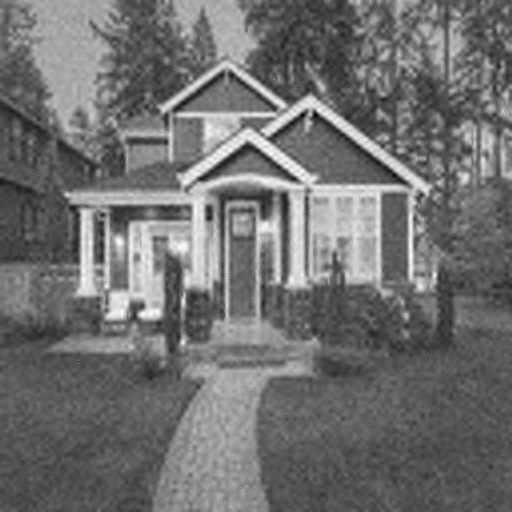
\includegraphics[width=3cm]{imgs/Thresholds/2_awt_soft_sym8_House.jpg}
    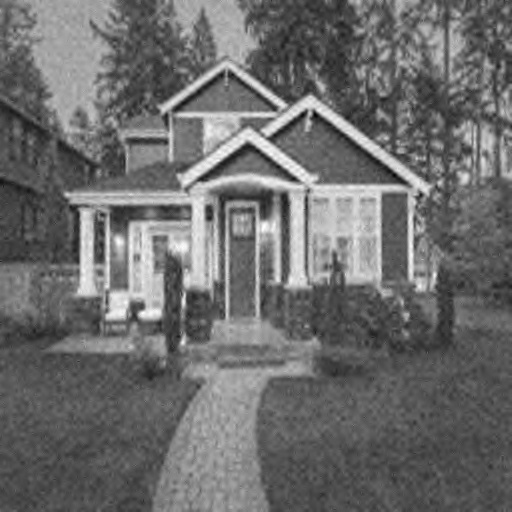
\includegraphics[width=3cm]{imgs/Thresholds/2_normal_soft_sym8_House.jpg}
    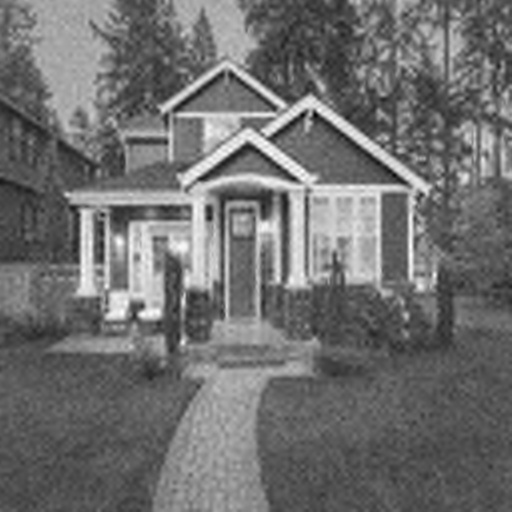
\includegraphics[width=3cm]{imgs/Thresholds/2_universal_soft_sym8_House.jpg}
    \\
    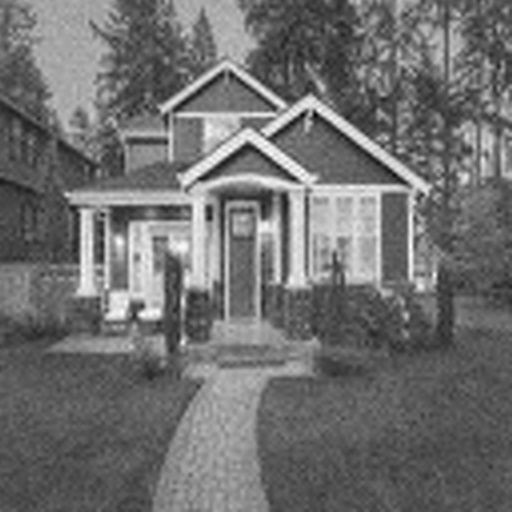
\includegraphics[width=3cm]{imgs/Thresholds/2_bayes_soft_sym8_House.jpg}
    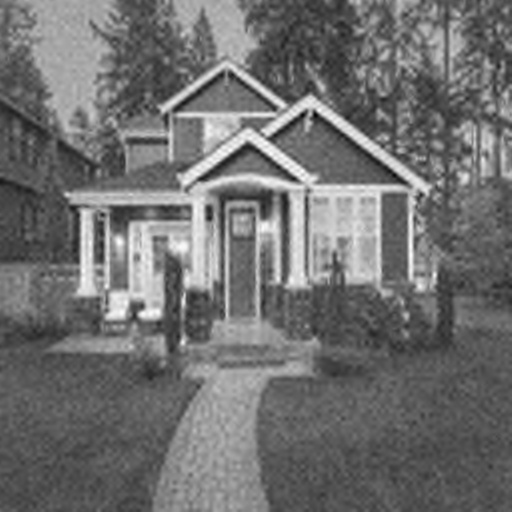
\includegraphics[width=3cm]{imgs/Thresholds/2_level_soft_sym8_House.jpg}
    

  \end{frame}

  \begin{frame}
    \frametitle{Comparacion de la Wavelet madre}
    \centering
    \begin{tabular}{lrrrr}
      \toprule
      {PSNR} &  noise &   haar &    db4 &   sym8 \\
      \midrule
      Lenna &  17.65 &  23.44 & 25.19 &  \bf{27.03} \\
      House &  19.87 &  \bf{26.38} &  24.78 &  25.58 \\
      Wave &  18.63 &  24.67 &  \bf{26.87} &  26.70 \\
      \bottomrule
      \end{tabular}
  
      \begin{tabular}{lrrrr}
        {SSIM} &  noise &   haar &    db4 &   sym8 \\
        \midrule
        Lenna &  0.518 &  0.819 &  0.853 &  \bf{0.856} \\
        House &  0.620 &  0.848 &  0.875 &  \bf{0.882} \\
        Wave &  0.586 &  0.805 &  0.836 &  \bf{0.839} \\
        \bottomrule
        \end{tabular}
  \end{frame}

  \begin{frame}
    \frametitle{Comparacion de la Wavelet madre - db4}
    
    \centering
    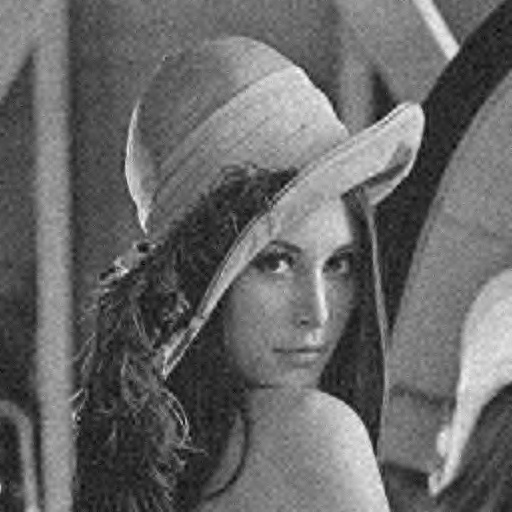
\includegraphics[width=6cm]{imgs/Wavelets/2_normal_soft_db4_Lenna.jpg}
   
  
  \end{frame}

  \begin{frame}
    \frametitle{Comparacion de la Wavelet madre - haar}
    
    \centering
    
    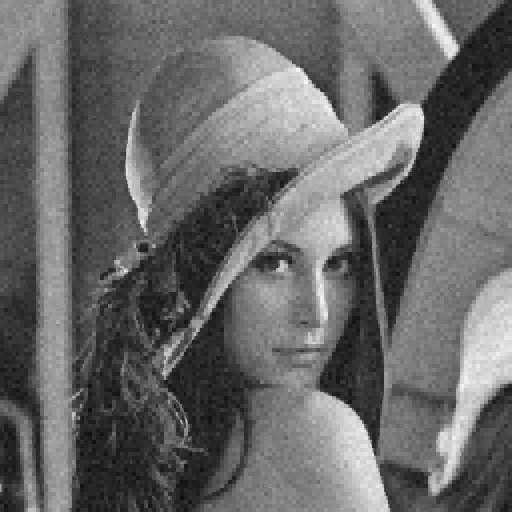
\includegraphics[width=6cm]{imgs/Wavelets/2_normal_soft_haar_Lenna.jpg}
    

  
  \end{frame}

  \begin{frame}
    \frametitle{Comparacion de la Wavelet madre - sym8}
    
    \centering
    
    
    \includegraphics[width=6cm]{imgs/Wavelets/2_normal_soft_sym8_Lenna.jpg}

  
  \end{frame}

  \begin{frame}
    \frametitle{Parametros optimos}
    \centering
    \begin{tabular}{llll}
      \toprule
      level & wavelet & mode & umbral \\
      \midrule 
      2 & sym8 & soft & normal \\
      \bottomrule
    \end{tabular}
  
  \end{frame}

  \subsection{Comparacion de filtros}

  \begin{frame}
    \frametitle{Resultado del filtrado}
  
    
  
  \end{frame}

  \section{Conclusiones}

\end{document}
